\chapter{Modelo de Casos de Uso}
\label{sec-casos-de-uso}
\vspace{-1cm}

% Define contador e identificador para casos de uso.
% Usar \UC\label{rf-nome-do-label} para cada caso de uso definido.
\newcounter{uccount}
\renewcommand*\theuccount{UC-\arabic{uccount}}
\newcommand*\UC{\refstepcounter{uccount}\theuccount}
\setcounter{uccount}{0}

\vitor{Listar e descrever os atores na Tabela~\ref{tbl-casos-de-uso-atores}. Para cada subsistema (se houver) ou para o sistema como um todo (se for um sistema simples), apresentar o diagrama de casos de uso (ex.: Figura~\ref{fig-casos-de-uso-subsistema-primeiro}) e a tabela que relaciona os casos de uso com as estórias de usuário (ex.: Tabela~\ref{tbl-casos-de-uso-subsistema-primeiro})).}

O modelo de casos de uso provê uma visão geral das funcionalidades do sistema, relacionando-as com seus respectivos atores. Os atores identificados no contexto deste projeto estão descritos na Tabela~\ref{tbl-casos-de-uso-atores}.

% Tabela de atores.
\begin{longtable}{|p{3cm}|p{12cm}|}
	\caption{Descrição dos atores envolvidos nos casos de uso.}
	\label{tbl-casos-de-uso-atores} \\\hline 
	
	% Cabeçalho e repetição do mesmo em cada nova página. Manter como está.
	\rowcolor{lightgray}
	\textbf{Ator} & \textbf{Descrição} \\\hline		
	\endfirsthead
	\hline
	\rowcolor{lightgray}
	\textbf{Ator} & \textbf{Descrição} \\\hline		
	\endhead
	
	% Especificar os atores abaixo, substituindo os exemplos.
	Ator 01 & Descrição do ator 01. \\\hline
	
	Ator 02 & Descrição do ator 02. \\\hline
	
	Ator 03 & Descrição do ator 03. \\\hline
\end{longtable}

A seguir, são apresentados os diagramas de casos de uso organizados por subsistema.



% Definir uma subseção para cada subsistema.	
\section{Subsistema 01}
\label{sec-casos-de-uso-subsistema-primeiro}

A Figura~\ref{fig-casos-de-uso-subsistema-primeiro} apresenta o diagrama de casos de uso do subsistema 01. Em seguida, a Tabela~\ref{tbl-casos-de-uso-subsistema-primeiro} indica a relação entre os casos de uso e as estórias de usuário, ou seja, quais requisitos do sistema cada caso de uso deve satisfazer.

\begin{figure}[h]
	\centering
	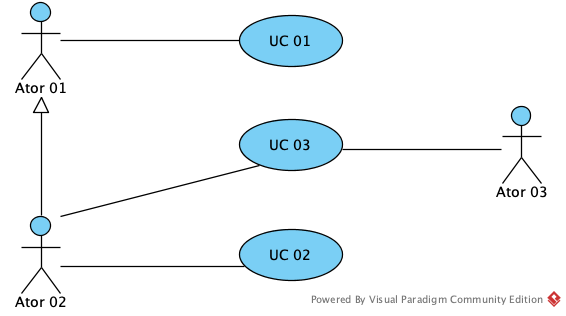
\includegraphics[width=.7\textwidth]{figuras/fig-casos-de-uso-subsistema-primeiro.png}
	\caption{Diagrama de Casos de Uso do subsistema 01.}
	\label{fig-casos-de-uso-subsistema-primeiro}
\end{figure}

\begin{longtable}{|c|p{10cm}|p{2.2cm}|}
	\caption{Relação entre os casos de uso do subsistema 01 e as estórias de usuário.}
	\label{tbl-casos-de-uso-subsistema-primeiro} \\\hline 
	
	% Cabeçalho e repetição do mesmo em cada nova página. Manter como está.
	\rowcolor{lightgray}
	\textbf{Id} & \textbf{Nome} & \textbf{Requisitos}\\\hline	
	\endfirsthead
	\hline
	\rowcolor{lightgray}
	\textbf{Id} & \textbf{Nome} & \textbf{Requisitos} \\\hline	
	\endhead
	
	\UC\label{uc-nucleo-installSystem} & UC 01
	& \ref{us-exemplo-generico}
	\\\hline
	
	\UC\label{uc-nucleo-login} & UC 02
	& \ref{us-exemplo-cadastro}
	\\\hline
	
	\UC\label{uc-nucleo-createAccount} & UC 03
	& \ref{us-exemplo-consulta}
	\\\hline
\end{longtable}

\FloatBarrier



% Definir uma subseção para cada subsistema.	
\section{Subsistema 02}
\label{sec-casos-de-uso-subsistema-segundo}

Etc...

\FloatBarrier
